% ============================================================================
% Class Declaration
% ============================================================================
\documentclass[
        mode = handout,     % Projector = one bullet at a time, Handout = all
        font-size=14pt,     % Only accepts 9, 10, 12, 14, 17, 20
        pdfusetitle         % Pulls \title property from document
    ]
    {ltx-talk}              % ltx-talk class

% ============================================================================
% Custom Colors
% ============================================================================
\usepackage[table]{xcolor}
% Colors from the Baker College Style Guide
\definecolor{BakerADARed}{RGB}{231, 0, 46}
\definecolor{HoneyYellow}{RGB}{255, 196, 0}
\definecolor{UpNorthGreen}{RGB}{114, 191, 68}
\definecolor{LakeBlue}{RGB}{134, 183, 227}
\definecolor{BakerADI}{RGB}{58, 98, 170}
\definecolor{BakerCIM}{RGB}{217, 35, 47}
\definecolor{BakerBlack}{RGB}{31, 34, 40}
\definecolor{BakerWhite}{RGB}{255, 255, 255}
\definecolor{BakerRed}{RGB}{239, 0, 48}
\definecolor{Abbey}{RGB}{80, 82, 88}
\definecolor{RollingStone}{RGB}{121, 124, 126}
\definecolor{HitGray}{RGB}{165, 169, 172}
\definecolor{Iron1}{RGB}{201, 206, 209}
\definecolor{Iron}{RGB}{222, 225, 226}
\definecolor{BlackHaze1}{RGB}{237, 240, 240}
\definecolor{BlackHaze}{RGB}{245, 247, 247}

% ============================================================================
% Document Data
% ============================================================================
\title{\PresTitle}
\author{\PresAuthor}
\institute{\PresInstitute}
\date{\PresDate}

%Set up the hyperlink colors
\hypersetup{colorlinks,
    linkcolor=BakerBlack,
    urlcolor=BakerADARed,
    pdfauthor = {\PresAuthor},
    %pdftitle = {\PresentationTopic},   % Title is pulled directly
    pdfsubject = {\PresSubtitle},
    pdfkeywords = {\Keywords},
    pdfcreator = {LaTeX with hyperref package},
    pdfproducer = {LuaLaTeX}
    }

% Map your custom style guide colors to the progress bar aliases
\colorlet{pbcomplete}{BakerADARed}
\colorlet{pbincomplete}{Iron}

\usepackage[most]{tcolorbox}

% ============================================================================
% Footer Format
% ============================================================================
\EditInstance{footer}{std}{
  color         = Abbey,
  separator     = \hfill,
  element-order = {title, institute, framenumber},
  right-hspace  = 3mm,
  left-hspace   = 3mm,
}

% \DeclareInstance{footer}{empty}{
%   element-order = {}
% }

% ============================================================================
% Progress Bar Toggles & Helper Macros
% ============================================================================
\usepackage{xfp}        % Needed for floating point math
\newif\ifprogressbar    % Used to determine whether or not to show the bar
\progressbartrue        % Set the bar to true at the start

% Helper macro to automatically turn off the progress bar inside title/section frames
\newcommand{\makeblindframe}[1]{%
  \progressbarfalse
  #1%
  \progressbartrue
}

% ============================================================================
% Custom Page Formats
% ============================================================================
\let\oldmaketitle\maketitle         % Backup the original maketitle command
\let\oldsection\section             % Backup the original section command
\let\oldsubsection\subsection       % Backup the original subsection command

\makeatletter
\renewcommand{\maketitle}{%
\makeblindframe{%
  \disableglobalbackground
  \slidebackground{BakerPresentation_TitleBackground}%
  \color{white}%
  %\UseInstance{footer}{wallpaper}
  \begin{frame}[wallpaper]
    \vspace*{1in}%
      \begin{tcolorbox}[
          enhanced,
          colback=black,       
          colframe=black,      
          opacityfill=0.25,       
          arc=6pt,                
          boxrule=0pt,            
          left=20pt, right=20pt,  
          top=20pt, bottom=20pt,
          width=0.80\textwidth,   
          halign=left             
      ]
          \color{white}%
          % Title (Always visible)
          {\large\bfseries\sffamily \@title}\\[0.5em]%
          
          % Conditional Subtitle
          \ifx\PresSubtitle\empty
          \else
            {\normalsize\sffamily \PresSubtitle}\\[0.5em]%
          \fi
          
          % High-contrast divider line
          {\color{white!80}\rule{0.3\textwidth}{0.8pt}}\\[0.5em]%
          
          % Author (Always visible)
          {\small\sffamily \@author}\\%
          
          % Conditional Institute
          \ifx\PresInstitute\empty
          \else
            {\small\sffamily \PresInstitute}\\%
          \fi
          
          % Conditional Date
          \ifx\PresDate\empty
          \else
            {\small\sffamily \@date}\\%
          \fi
      \end{tcolorbox}%
      \vfill     
  \end{frame}%
  \enableglobalbackground{BG}%
  \color{black}%
  %\UseInstance{footer}{std}
}%
}
\makeatother

% Create a variable container to hold the current section title
\newcommand{\currentsectiontitle}{}

% Redefine \section to take 1 argument (the title)
\renewcommand{\section}[1]{%
\makeblindframe{%
  \renewcommand{\currentsectiontitle}{#1}%
  \disableglobalbackground
  \slidebackground{BakerPresentation_SectionBackground}%
  \begin{frame}
    \vfill
    %\vspace*{0.625in}%
    \begin{tcolorbox}[
        enhanced,
        colback=black,       
        colframe=black,      
        opacityfill=0.25,       
        arc=6pt,                
        boxrule=0pt,            
        left=20pt, right=20pt,  
        top=20pt, bottom=20pt,
        width=0.80\textwidth,   
        halign=left             
    ]
        \color{white}%
        {\large\bfseries\sffamily #1}\\[0.5em]%   
    \end{tcolorbox}%
    \vfill 
  \end{frame}%
  \oldsection{#1}%
  \enableglobalbackground{BG}%

  % This will be used for an auto TOC at every section
  % Right now ltx-talk TOC is still in development
  % Once it comes a little further along this can be used
  % \begin{frame}
  %       \frametitle{Section Overview}
  %       \tableofcontents[sections=\thesection]
  %   \end{frame}%
}%
}

% Redefine \subsection to take 1 argument
\renewcommand{\subsection}[1]{%
\makeblindframe{%
  \disableglobalbackground
  \slidebackground{BakerPresentation_SectionBackground}%
  \begin{frame}
    \vfill
    %\vspace*{0.25in}% 
    \begin{tcolorbox}[
        enhanced,
        colback=black,       
        colframe=black,      
        opacityfill=0.25,       
        arc=6pt,                
        boxrule=0pt,            
        left=20pt, right=20pt,  
        top=20pt, bottom=20pt,
        width=0.80\textwidth,   
        halign=left             
    ]
        \color{white}%
        {\large\bfseries\sffamily\currentsectiontitle}\\[0.5em]%
        {\normalsize\sffamily #1}%
    \end{tcolorbox}%
    \vfill 
  \end{frame}%
  \oldsubsection{#1}%
  \enableglobalbackground{BG}%
}%
}

%Set the fonts to use NeueHaas Grotesk
\setsansfont{NHaasGroteskTXPro-}[
    Path=../../NeueHaasGroteskFiles/,
    Scale=1.0,
    Extension = .ttf,
    UprightFont=*55Rg,
    BoldFont=*75Bd,
    ItalicFont=*56It,
    BoldItalicFont=*76BdIt
    ]

% Force the document default family to Sans-Serif
\renewcommand{\familydefault}{\sfdefault}

\usepackage{mathtools} % Load BEFORE unicode math settings
\setmathfont{Fira Math}[Scale=MatchLowercase] 

% 1. Turn global background ON
\newcommand{\enableglobalbackground}[1]{%
  \AddToHook{shipout/background}[mybg]{%
    \put(0, -\paperheight){%
      \includegraphics[width=\paperwidth, height=\paperheight, artifact]{#1}%
    }%
  }%
}

% 2. Turn global background OFF
\newcommand{\disableglobalbackground}{%
  \RemoveFromHook{shipout/background}[mybg]%
}

\newcommand{\slidebackground}[1]{%
  \AddToHookNext{shipout/background}{%
    \put(0, -\paperheight){%
      \includegraphics[width=\paperwidth, height=\paperheight, artifact]{#1}%
    }%
  }%
}

% --- GLOBAL BULLET OVERRIDES ---
\renewcommand{\labelitemi}{\color{BakerBlack}\Large\textbullet}
\renewcommand{\labelitemii}{\color{BakerBlack}\large\textbullet}
\renewcommand{\labelenumi}{\color{BakerBlack}\bfseries\arabic{enumi}.}
\renewcommand{\labelenumii}{\color{BakerBlack}\bfseries\alph{enumii})}

% Global override for ltx-talk slide titles
\EditInstance{frametitle}{header}{
    font = \rule{0pt}{1.5cm}\bfseries\Large,
}

\EditInstance{header}{std}{
    font = \bfseries\huge,
    color = BakerBlack,
}

\usepackage[americanvoltages]{circuitikz}
\usepackage{pgfplots}
\usepackage{pgf-pie}

\usetikzlibrary{
    intersections, 
    fillbetween,
    patterns,
    decorations.pathreplacing,
    decorations.pathmorphing,
    decorations.text,
    decorations.markings,
    arrows.meta,
    arrows,
    shapes,
    shapes.geometric,
    shadows,
    calligraphy,
    backgrounds,
    intersections,
    calc,
    math,
    positioning
    }

\tikzset{middlearrow/.style={
        decoration={markings, 
        mark= at position 0.5 with {\arrow{#1}},
        },
        postaction={decorate}
    }
}

\pgfplotsset{compat=1.18}

\pgfdeclarelayer{ft}
\pgfdeclarelayer{bg}
\pgfsetlayers{bg, main, ft}

\newcommand{\hexpic}[4][]{%
  \begin{tikzpicture}[baseline=(hex.base)]
    \node (hex) [
      draw=white, 
      minimum size=#2, 
      regular polygon, 
      regular polygon sides=6, 
      rotate=90,
    ] {};
    \begin{scope}
      \clip (hex.corner 1) -- (hex.corner 2) -- (hex.corner 3) -- 
            (hex.corner 4) -- (hex.corner 5) -- (hex.corner 6) -- cycle;
      \node at (hex.center) [#1] {
        \includegraphics[height=#2, alt={#3}]{#4}
      };
    \end{scope}
  \end{tikzpicture}
}

% % ============================================================================
% % Progress Bar Logic 
% % ============================================================================
% \makeatletter               
% \AddToHook{shipout/background}{%
%   \ifprogressbar
%     % Read ltx-talk's internal frame counters safely
%     \edef\currentframe{\@framenumber}%
%     \edef\totalframes{\@totalframes}%
    
%     % Fallback checks: If the document hasn't fully compiled yet, default to 1
%     \ifx\currentframe\empty\def\currentframe{1}\fi
%     \ifx\totalframes\empty\def\totalframes{1}\fi
    
%     % Draw the progress bar if we have a valid total frame count
%     \ifnum\totalframes>1\relax
%       % Compute fraction width: (current - 1) / (total - 1)
%       \edef\pbfraction{\fpeval{(\currentframe - 1) / (\totalframes - 1)}}%
%       \edef\completewidth{\fpeval{\pbfraction * \paperwidth}}%
%       \edef\incompletewidth{\fpeval{\paperwidth - \completewidth}}%
      
%       % Render full-width progress bar at the top edge
%       \put(0cm, -0.1cm){%
%         \color{pbcomplete}\rule{\completewidth pt}{2pt}%
%         \color{pbincomplete}\rule{\incompletewidth pt}{2pt}%
%       }%
%     \fi
%   \fi
% }
% \makeatother

\pretocmd{\tableofcontents}{\begin{minipage}{\textwidth} \linespread{1.4}}{}{}
\apptocmd{\tableofcontents}{\end{minipage}}{}{}

%Biber not functional in ltx-talk as of 2026-05-29
%Package that allows the creation of bibliographies
\usepackage[
    backend=biber,
    style=authoryear,
    sorting=none,
    %entryhead=false
    ]{biblatex}

%Load the bibliography file
\addbibresource{../../reference.bib}

\defbibheading{bibslide}{References}

\newcolumntype{L}[1]{>{\raggedright\let\newline\\\arraybackslash\hspace{0pt}}m{#1}}
\newcolumntype{C}[1]{>{\centering\let\newline\\\arraybackslash\hspace{0pt}}m{#1}}
\newcolumntype{R}[1]{>{\raggedleft\let\newline\\\arraybackslash\hspace{0pt}}m{#1}}

%All of the graphics are in a seperate folder, this makes it so the folder doesn't have to be repeated every time
\graphicspath{
  {../../assets/images}
  {../../assets/diagrams}
  {../../assets/plots}
}

\makeatletter
% New counter to hold the custom "max frames" for the progress bar
\newcommand{\pb@maxtotal}{1}

% Read the custom total from the .aux file if it exists
\AtBeginDocument{%
  \ifdefined\pb@storedtotal
    \let\pb@maxtotal\pb@storedtotal
  \else
    % Fallback to standard total if our custom hook hasn't run yet
    \edef\pb@maxtotal{\@totalframes}%
  \fi
}

% Custom Appendix command that caps the progress bar and turns it off
\newcommand{\talkappendix}{%
  % 1. Write the CURRENT frame number to the .aux file as the progress total
  \immediate\write\@auxout{\string\gdef\string\pb@storedtotal{\@framenumber}}%
  % 2. Turn off the progress bar for all subsequent appendix slides
  \progressbarfalse
}
\makeatother

% ============================================================================
% Progress Bar Logic 
% ============================================================================
\makeatletter               
\AddToHook{shipout/background}{%
  \ifprogressbar
    % Read ltx-talk's internal frame counter safely
    \edef\currentframe{\@framenumber}%
    \edef\totalframes{\pb@maxtotal}% Use our custom max total instead
    
    % Fallback checks: If the document hasn't fully compiled yet, default to 1
    \ifx\currentframe\empty\def\currentframe{1}\fi
    \ifx\totalframes\empty\def\totalframes{1}\fi
    
    % Draw the progress bar if we have a valid total frame count
    \ifnum\totalframes>1\relax
      % Compute fraction width: (current - 1) / (total - 1)
      \edef\pbfraction{\fpeval{(\currentframe - 1) / (\totalframes - 1)}}%
      
      % Guard rails to prevent the bar from overshooting 100% on a first compile
      \ifdim\pbfraction pt>1pt\def\pbfraction{1}\fi 
      
      \edef\completewidth{\fpeval{\pbfraction * \paperwidth}}%
      \edef\incompletewidth{\fpeval{\paperwidth - \completewidth}}%
      
      % Render full-width progress bar at the top edge
      \put(0cm, -0.1cm){%
        \color{pbcomplete}\rule{\completewidth pt}{2pt}%
        \color{pbincomplete}\rule{\incompletewidth pt}{2pt}%
      }%
    \fi
  \fi
}
\makeatother

% 1. Globally shrink all caption components right as the caption engine fires
\AddToHook{cmd/@makecaption/before}{\footnotesize}

% 2. Declare and assign a blank plug to the kernel's caption label socket
\NewSocketPlug{caption/label}{nolabel}{}
\AssignSocketPlug{caption/label}{nolabel}

\usepackage{adjustbox}

\usepackage{amssymb}
\usepackage{amsmath}

\newcommand{\ccwplus}{%
  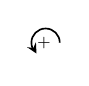
\begin{tikzpicture}[baseline=(char.base)]
    \node(char) at (0,0) {\(\scriptscriptstyle +\)};
    \draw[->, >=stealth, semithick] (0.2,0) arc (0:230:0.18cm);
  \end{tikzpicture}%
}

\usepackage{animate}

\usepackage{calc} % Optional, but helpful for layout

\newcommand{\tikztodo}[3][0.8\textwidth]{%
  \begin{center}
    \fbox{%
      \parbox[c][#2][c]{#1}{%
        \centering
        \textbf{\textcolor{red}{TODO: TikZ Diagram}}\\[0.5em]
        \small #3%
      }%
    }%
  \end{center}%
}